\chapter{Resources}

\section{Hardware Architecture Overview}
\label{sec:hw_arch}

\begin{figure}[H]
\centering
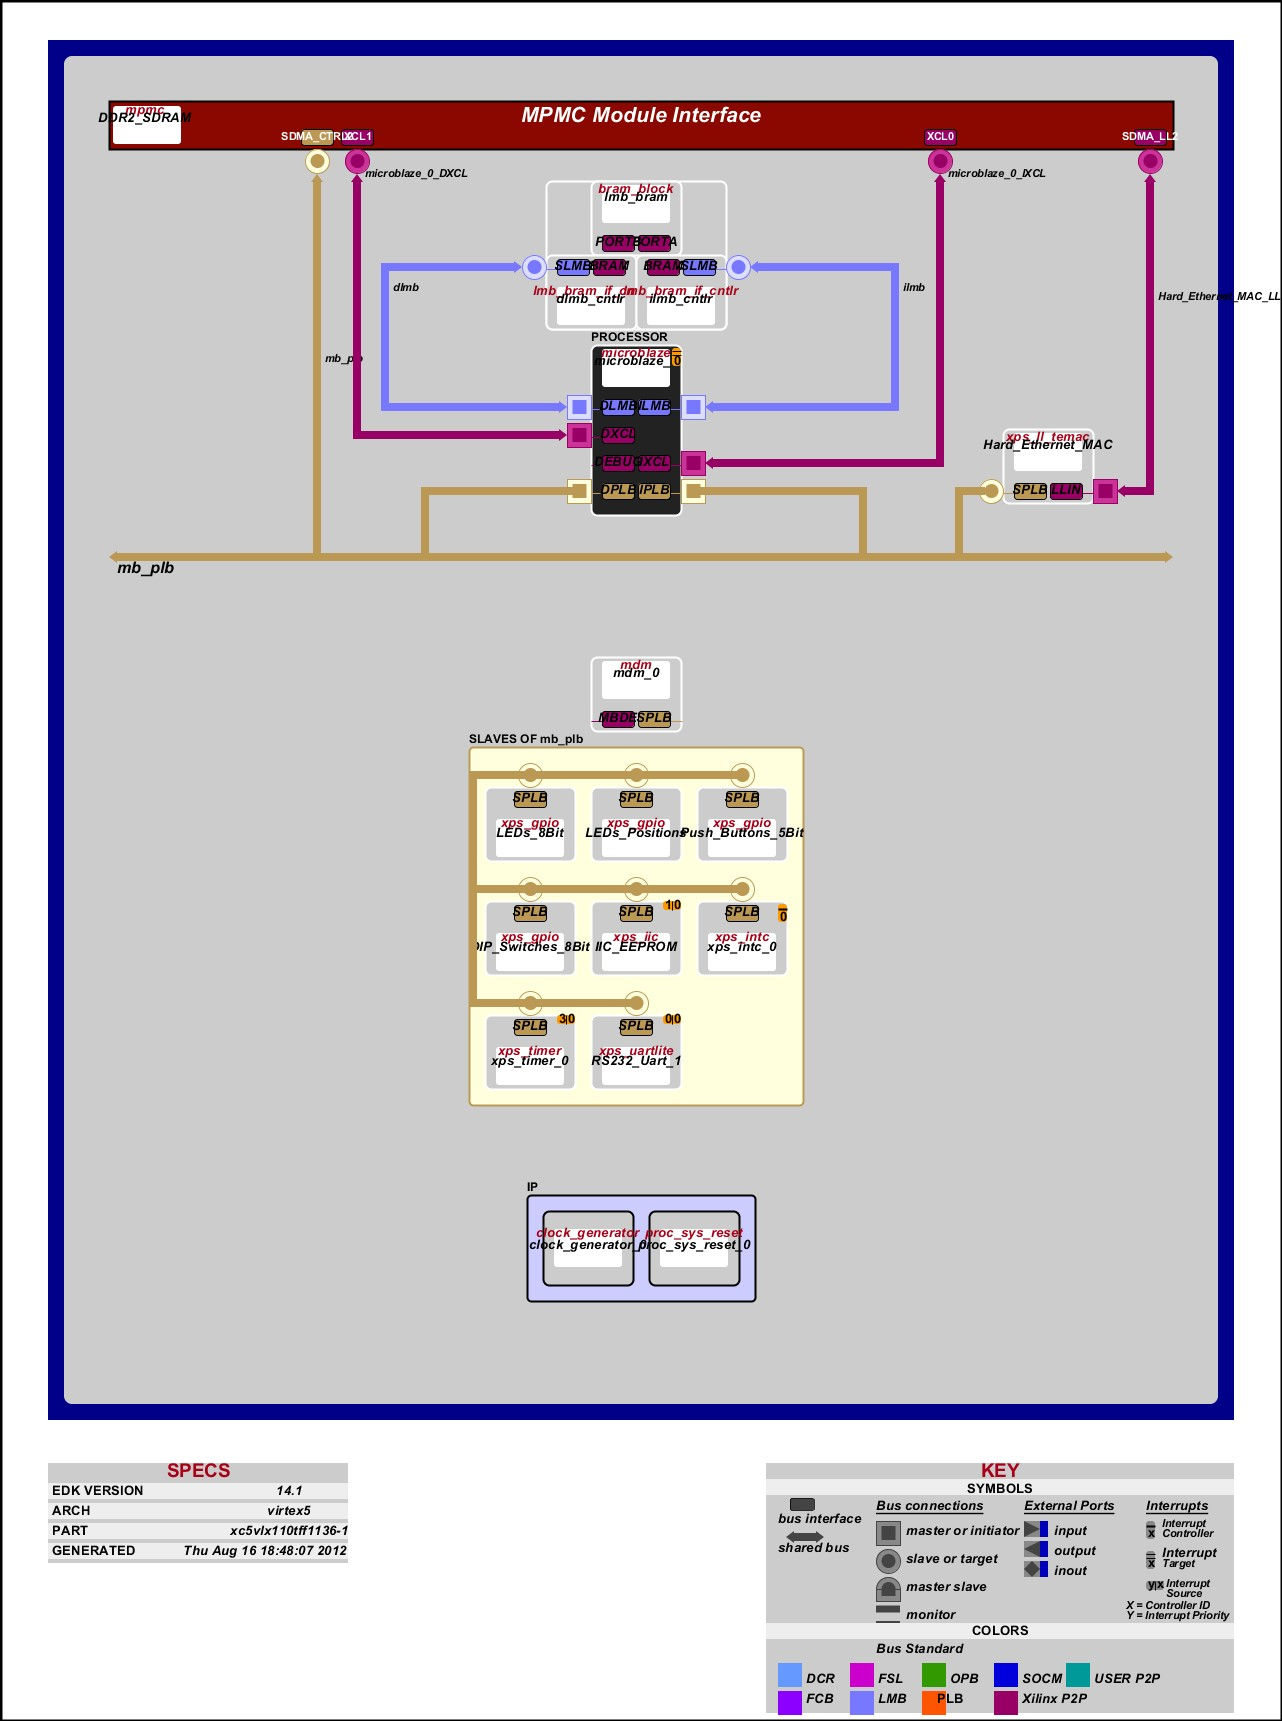
\includegraphics[width=0.9\textwidth]{images/system_blkd.jpg}
\end{figure}

\section{Hardware Project Configurations}

The configuration files contain more than 800 lines, being too much to include them directly in the project report. Therefore the \textit{Microprocessor Hardware Specification (mhs)} and \textit{User Constraint File (ucf)} files can be downloaded as part of the projects for \textit{\gls{xps}} and the \textit{Xilinx ISE Project Navigator} from the following address: \url{http://www.peschuster.de/ies-project/IesHttpProject-Hardware.zip}.
\\

\section{Linux Kernel Assets}

\subsection{Configuration}

The Linux kernel configuration file contains more than 1,200 lines and is therefore not included directly within this appendix, but can be downloaded together with all other scripts concerning the software part of this project from the following address: \url{http://www.peschuster.de/ies-project/IesHttpProject-Software.zip}.

Here are the configuration settings specific for the \textit{MicroBlaze} processor used in this project:

\begin{verbatim}
CONFIG_KERNEL_BASE_ADDR=0x50000000
CONFIG_XILINX_MICROBLAZE0_FAMILY="virtex5"
CONFIG_XILINX_MICROBLAZE0_USE_MSR_INSTR=1
CONFIG_XILINX_MICROBLAZE0_USE_PCMP_INSTR=1
CONFIG_XILINX_MICROBLAZE0_USE_BARREL=1
CONFIG_XILINX_MICROBLAZE0_USE_DIV=1
CONFIG_XILINX_MICROBLAZE0_USE_HW_MUL=2
CONFIG_XILINX_MICROBLAZE0_USE_FPU=0
CONFIG_XILINX_MICROBLAZE0_HW_VER="8.30.a"
\end{verbatim} 

\subsection{Patches}
\label{subsec:pvr_patch}

Path for correct recognition of the latest \textit{MicroBlaze} processor versions with enabled \gls{pvr}:

\begin{verbatim}
commit 9be0160c855d1740f392d74a90197421c1380946
Author: Peter Schuster <schuster.pe@gmail.com>
Date:   Sat Sep 8 19:48:56 2012 +0200

    Added new MicroBlaze versions.

diff --git a/arch/microblaze/kernel/cpu/cpuinfo.c b/arch/microblaze/kernel/cpu/cpuinfo.c
index 54194b2..783c7087 100644
--- a/arch/microblaze/kernel/cpu/cpuinfo.c
+++ b/arch/microblaze/kernel/cpu/cpuinfo.c
@@ -35,6 +35,8 @@ const struct cpu_ver_key cpu_ver_lookup[] = {
 	{"8.00.b", 0x13},
 	{"8.10.a", 0x14},
 	{"8.20.a", 0x15},
+        {"8.20.b", 0x16},
+        {"8.30.a", 0x17},
 	{NULL, 0},
 };
\end{verbatim}

The patch file "\texttt{new-microblaze-versions.patch}" is also included in the zip archive available at \url{http://www.peschuster.de/ies-project/IesHttpProject-Software.zip}.
\\

\section{Image files}

The \textit{bitstream} (\texttt{system.bit}) and Linux kernel image (\texttt{simpleImage.xupv5}) files for the \textit{Xilinx XUPV5-LX110T} board and described hardware system are available for download at \url{http://www.peschuster.de/ies-project/IesHttpProject-Images.zip}.


\section{SoC Environment Evaluation Program}
\label{sec:nginx-env-eval}

\textbf{C program}
\begin{verbatim}
#include <stdio.h>
#include <stdlib.h>
#include <signal.h>
#include "xparameters.h"
#include "xil_cache.h"

void print(char *str);

int main()
{
    #ifdef XPAR_MICROBLAZE_USE_ICACHE
        Xil_ICacheEnable();
    #endif
    #ifdef XPAR_MICROBLAZE_USE_DCACHE
        Xil_DCacheEnable();
    #endif

    print("Env analysis (size_of): \r\n \r\n");

    printf("size of int: %d \r\n", (int)sizeof(int));
    printf("size of long: %d \r\n", (int)sizeof(long));
    printf("size of long long: %d \r\n", (int)sizeof(long long));
    printf("size of void *: %d \r\n", (int)sizeof(void *));
    printf("size of sig_atomic_t: %d \r\n", (int)sizeof(sig_atomic_t));
    printf("size of size_t: %d \r\n", (int)sizeof(size_t));
    printf("size of off_t: %d \r\n", (int)sizeof(off_t));
    printf("size of time_t: %d \r\n", (int)sizeof(time_t));

    Xil_DCacheDisable();
    Xil_ICacheDisable();

    return 0;
}
\end{verbatim}

\textbf{Result}
\begin{verbatim}
size of int: 4
size of long: 4
size of long long: 8
size of void *: 4
size of sig_atomic_t: 4
size of size_t: 4
size of off_t: 4
size of time_t: 4
\end{verbatim}

\section{nginx patch: memory guard}
\label{appendix:memguard}

\begin{verbatim}
From 123fb80eea9fa7b3e6503c2d70a2eb9a32c33aca Mon Sep 17 00:00:00 2001
From: Peter Schuster <schuster.pe@gmail.com>
Date: Tue, 25 Dec 2012 23:25:41 +0100
Subject: [PATCH] Added a memory watch guard.

Implemented a watch guard checking remaining free system memory every
second and restarting worker processes if required.
---
 auto/options                       |    5 ++-
 auto/sources                       |    2 +
 auto/unix                          |    2 +
 build.sh                           |    1 +
 src/os/unix/ngx_process_cycle.c    |   27 +++++++++++++++++-
 src/os/unix/ngx_process_memguard.c |   53 ++++++++++++++++++++++++++++++++++++
 src/os/unix/ngx_process_memguard.h |    7 +++++
 7 files changed, 94 insertions(+), 3 deletions(-)
 create mode 100644 src/os/unix/ngx_process_memguard.c
 create mode 100644 src/os/unix/ngx_process_memguard.h

diff --git a/auto/options b/auto/options
index d405901..d1683ec 100644
--- a/auto/options
+++ b/auto/options
@@ -185,8 +185,9 @@ do
         --with-size-t=*)                 NGX_WITH_SIZE_T="$value"       ;;
         --with-off-t=*)                  NGX_WITH_OFF_T="$value"        ;;
         --with-time-t=*)                 NGX_WITH_TIME_T="$value"       ;;
-	--with-endian=*)                 NGX_WITH_ENDIAN="$value"   	;;
-	--with-sys-nerr=*)               NGX_WITH_NGX_SYS_NERR="$value" ;;
+        --with-endian=*)                 NGX_WITH_ENDIAN="$value"       ;;
+        --with-sys-nerr=*)               NGX_WITH_NGX_SYS_NERR="$value" ;;
+        --with-min-free-mem=*)           NGX_PROCESS_FREEMEM_MIN="$value";;
 
         --builddir=*)                    NGX_OBJS="$value"          ;;
 
diff --git a/auto/sources b/auto/sources
index cc19f8d..777d5ee 100644
--- a/auto/sources
+++ b/auto/sources
@@ -154,6 +154,7 @@ UNIX_DEPS="$CORE_DEPS $EVENT_DEPS \
             src/os/unix/ngx_socket.h \
             src/os/unix/ngx_os.h \
             src/os/unix/ngx_user.h \
+            src/os/unix/ngx_process_memguard.h \
             src/os/unix/ngx_process_cycle.h"
 
 # add to UNIX_DEPS
@@ -185,6 +186,7 @@ UNIX_SRCS="$CORE_SRCS $EVENT_SRCS \
             src/os/unix/ngx_setproctitle.c \
             src/os/unix/ngx_posix_init.c \
             src/os/unix/ngx_user.c \
+            src/os/unix/ngx_process_memguard.c \
             src/os/unix/ngx_process_cycle.c"
 
 POSIX_DEPS=src/os/unix/ngx_posix_config.h
diff --git a/auto/unix b/auto/unix
index ed4a1e3..fa86d0e 100755
--- a/auto/unix
+++ b/auto/unix
@@ -792,3 +792,5 @@ ngx_feature_test='struct addrinfo *res;
                   if (getaddrinfo("localhost", NULL, NULL, &res) != 0) return 1;
                   freeaddrinfo(res)'
 . auto/feature
+
+have=NGX_PROCESS_FREEMEM_MIN value=$NGX_PROCESS_FREEMEM_MIN . auto/define
\ No newline at end of file
diff --git a/build.sh b/build.sh
index 91d3408..192f214 100755
--- a/build.sh
+++ b/build.sh
@@ -58,6 +58,7 @@ export CROSS_COMPILE=microblaze-unknown-linux-gnu-
 	--with-size-t=4 \
 	--with-off-t=4 \
 	--with-time-t=4 \
+	--with-min-free-mem=10240 \
 	--with-cc-opt="-mxl-multiply-high -mno-xl-soft-mul -mno-xl-soft-div -mxl-barrel-shift -mxl-pattern-compare -mcpu=v8.30.a --static --sysroot=/home/peschuster/project/microblaze-unknown-linux-gnu/microblaze-unknown-linux-gnu/sys-root -g" > configure.log
 
 # --sysroot=/home/peschuster/project/microblaze-unknown-linux-gnu/microblaze-unknown-linux-gnu/sys-root
diff --git a/src/os/unix/ngx_process_cycle.c b/src/os/unix/ngx_process_cycle.c
index c9b0266..3b6af74 100644
--- a/src/os/unix/ngx_process_cycle.c
+++ b/src/os/unix/ngx_process_cycle.c
@@ -4,12 +4,14 @@
  * Copyright (C) Nginx, Inc.
  */
 
-
 #include <ngx_config.h>
 #include <ngx_core.h>
 #include <ngx_event.h>
 #include <ngx_channel.h>
 
+#ifdef NGX_PROCESS_FREEMEM_MIN
+#include <ngx_process_memguard.h>
+#endif
 
 static void ngx_start_worker_processes(ngx_cycle_t *cycle, ngx_int_t n,
     ngx_int_t type);
@@ -89,6 +91,7 @@ ngx_master_process_cycle(ngx_cycle_t *cycle)
     ngx_uint_t         n, sigio;
     sigset_t           set;
     struct itimerval   itv;
+    struct itimerval   itmem;
     ngx_uint_t         live;
     ngx_msec_t         delay;
     ngx_listening_t   *ls;
@@ -164,6 +167,17 @@ ngx_master_process_cycle(ngx_cycle_t *cycle)
             }
         }
 
+        #ifdef NGX_PROCESS_FREEMEM_MIN
+        itmem.it_interval.tv_sec = 0;
+        itmem.it_interval.tv_usec = 0;
+        itmem.it_value.tv_sec = 1;
+        itmem.it_value.tv_usec = 0;
+
+        if (setitimer(ITIMER_REAL, &itmem, NULL) == -1) {
+            ngx_log_error(NGX_LOG_ALERT, cycle->log, ngx_errno, "setitimer() failed");
+        }
+		#endif
+
         ngx_log_debug0(NGX_LOG_DEBUG_EVENT, cycle->log, 0, "sigsuspend");
 
         sigsuspend(&set);
@@ -173,6 +187,17 @@ ngx_master_process_cycle(ngx_cycle_t *cycle)
         ngx_log_debug1(NGX_LOG_DEBUG_EVENT, cycle->log, 0,
                        "wake up, sigio %i", sigio);
 
+        #ifdef NGX_PROCESS_FREEMEM_MIN
+        if (ngx_sigalrm == 1) {
+            ngx_sigalrm = 0;
+			
+            ngx_log_debug0(NGX_LOG_DEBUG_EVENT, cycle->log, 0, "checking free mem");
+            if (ngx_master_process_memguard_triggered(NGX_PROCESS_FREEMEM_MIN) != 0) {
+			    ngx_reconfigure = 1;
+            }
+        }
+        #endif
+
         if (ngx_reap) {
             ngx_reap = 0;
             ngx_log_debug0(NGX_LOG_DEBUG_EVENT, cycle->log, 0, "reap children");
diff --git a/src/os/unix/ngx_process_memguard.c b/src/os/unix/ngx_process_memguard.c
new file mode 100644
index 0000000..581510c
--- /dev/null
+++ b/src/os/unix/ngx_process_memguard.c
@@ -0,0 +1,53 @@
+
+#include <stdio.h>
+#include <string.h>
+#include <ngx_process_memguard.h>
+
+const unsigned MAXLINE=9999;
+
+char* _ngx_process_memguard_trim_ws(char *line)
+{
+    return line + strspn(line, " \t");
+}
+
+char* _ngx_process_memguard_find_line(char *line)
+{
+	const char* match = "MemFree:";
+	const int match_len = 8;
+    char *p;
+
+    p = _ngx_process_memguard_trim_ws(line);
+	
+    return (strncmp(p, match,  match_len) == 0) ? (p + match_len) : NULL;
+}
+
+char ngx_master_process_memguard_triggered(long min_mem)
+{
+    char *p, *pend;
+    char line[MAXLINE];
+    long fmem = 0;
+    FILE *proc_meminfo = fopen("/proc/meminfo", "r");
+
+    if (!proc_meminfo) {
+        return 0;
+	}
+	
+	while ((p = fgets(line, MAXLINE, proc_meminfo))) {
+		if ((p = _ngx_process_memguard_find_line(line))) {
+			
+			 // check last char for newline terminator
+            pend = p + strlen(p) - 1;
+            if (*pend == '\n') *pend=0;
+            
+			p = _ngx_process_memguard_trim_ws(p);			
+			sscanf(p, "%ld", &fmem);
+	
+			fclose(proc_meminfo);
+			
+			return (fmem * 1024) < min_mem;
+        }
+    }
+	
+	fclose(proc_meminfo);	
+	return 0;	
+}
diff --git a/src/os/unix/ngx_process_memguard.h b/src/os/unix/ngx_process_memguard.h
new file mode 100644
index 0000000..0a3d035
--- /dev/null
+++ b/src/os/unix/ngx_process_memguard.h
@@ -0,0 +1,7 @@
+
+#ifndef _NGX_PROCESS_MEMGUARD_H_INCLUDED_
+#define _NGX_PROCESS_MEMGUARD_H_INCLUDED_
+
+char ngx_master_process_memguard_triggered(long min_mem);
+
+#endif /* _NGX_PROCESS_MEMGUARD_H_INCLUDED_ */
-- 
1.7.8.msysgit.0

\end{verbatim}


\section{C\# Load Test Console Application}
\label{appendix:csharp-load}

\begin{verbatim}
using System;
using System.Net;
using System.Threading;
using System.Threading.Tasks;

class Program
{
    static void Main(string[] args)
    {
        while (true)
        {
            Console.WriteLine("Specify params. Form: [number]:[threads]");
            string input = Console.ReadLine();

            if (string.IsNullOrWhiteSpace(input))
                return;

            string[] p = input.Split(':');
            int req = int.Parse(p[0]);
            if (req <= 0)
                return;

            long count = 0;
            DateTime start = DateTime.Now;

            int parallel = int.Parse(p[1]);
            string baseUrl = "http://192.168.2.125/10K.html?id=";
            var parellelOptions = new ParallelOptions { MaxDegreeOfParallelism = parallel };

            Parallel.For(0, req, parellelOptions, i =>
            {
                var http = HttpWebRequest.CreateHttp(baseUrl + i);
                    
                using (http.GetResponse())
                {
                }

                double c = Interlocked.Increment(ref count);

                if (i % 10 == 0)
                {
                    Console.WriteLine(
                        "{0, 8} {1:0.000}", 
                        c, 
                        c / (DateTime.Now - start).TotalSeconds);
                }
            });
        }
    }
}
\end{verbatim}